\section{Introduction}\label{sec:Introduction}

%As big data techniques and infrastructures are being applied to facilitate and accelerate the processing of big data with formidable size, people are putting forward eager requests on (quasi-)real-time processing of big datasets yet with exploding volumes, while meeting the (quasi-)real-time processing requests of big datasets is held back by the disk-based storage subsystem, because of the expanding tremendous performance gap lying between magnetic disks and processing units.

Memory caching \textcolor{red}{plays} a crucial role in bridging the performance gap between \textcolor{red}{storage subsystems and computing frameworks, which gradually becomes the determinant of whether processing units of big data platforms could work at wire speed to satisfy people's growing computing requirements.}
As more and more time-critical applications commence employing memory to cache datasets, big data clusters \textcolor{red}{are usually} shared by multiple computing \textcolor{red}{frameworks}, applications or end users, and  there exists intense competition for memory cache resources, especially on small clusters which are supposed to 
\textcolor{red}{process comparably big datasets as large clusters do, yet with tightly limited resources.}
Consequently implementing effective and adaptive management on memory cache resources becomes increasingly important for the efficient running of big data clusters, especially for small/medium enterprises \textcolor{red}{who} could only afford to build non-big clusters. Applying existing on-demand caching strategies on small shared clusters inevitably results in frequent cache thrashings when the conflicts of simultaneous cache resource demands are not mediated, \textcolor{red}{leading to deterioration in overall cluster efficiency.}
The principal reason is that aggressively caching massive number of data blocks of big datasets on demand causes \textcolor{red}{constant block replacement in cache, and thus conversely exacerbates resource competition.}

%\begin{figure}[!htb]
%\centering
%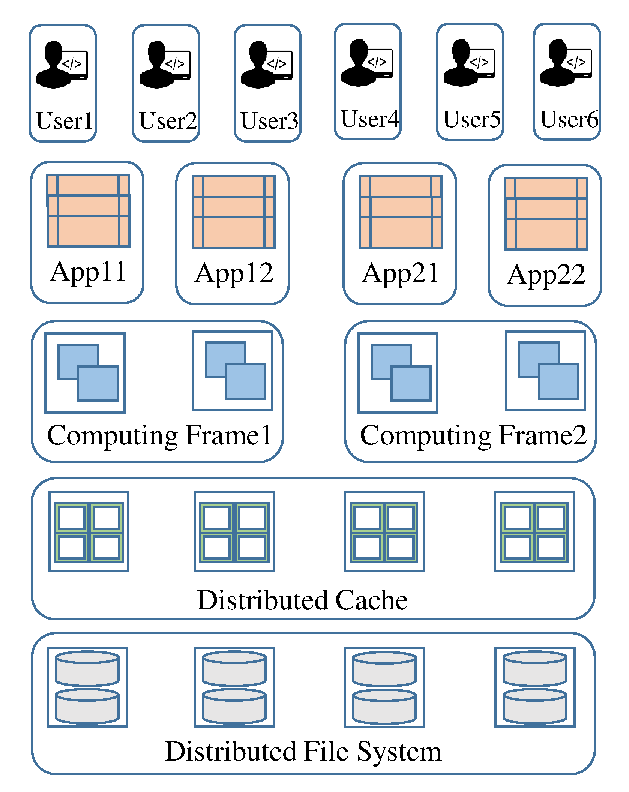
\includegraphics[width=0.4\textwidth]{figures-final/Hierarchy.eps}
%\caption{Big data application hierarchies.}
%\label{fig:hierarchy}
%\end{figure}

%Intense competition for computational resources would do no harm to the clusters' running efficiency, while intense competitions for memory cache resources may incur frequent cache thrashings if cache resource demands are not coordinated, which would engender tremendous harm to the clusters' running efficiency.

%Applying existing on-demand caching strategies, which cache in data blocks once they are accessed, on small shared clusters could not prevent cache thrashings when the conflicts of simultaneous cache resource demands are not mediated. The principal reason is that aggressively caching massive number of data blocks of big datasets on demand causes constantly block replacement in cache, and thus exacerbates the competition of memory cache resources when these resources are in strong need.

\textcolor{red}{Web or traditional OLTP database applications usually produces vast difference in range or block "hotness" regarding access recency and frequency. Though in big data applications, input files are usually scanned as a whole for data processing and all blocks reveal almost equal "hotness".}
%Unlike Web or traditional OLTP database applications, where various ranges or blocks of the same dataset may possess \textcolor{red}{vast} different "hotness", regarding access recency and frequency of blocks, big data applications usually scan their input files for data processing as a whole, and all blocks of a file thus possess almost the same level of "hotness". 
\textcolor{red}{On the other hand}, traditional \textcolor{red}{system-level} or database-level data caching is executed on small data units (i.e. 8KB-sized pages), while big data caching is executed on \textcolor{red}{much larger} units(i.e. 256MB-sized blocks). So the cost of caching in/out a data unit \textcolor{red}{in big data scenarios} far exceeds that \textcolor{red}{of} traditional data caching. Accordingly, traditional caching may have millions of \textcolor{red}{cache slots}, and this makes hotter data less likely cached out by colder data; while big data caching may only have thousands of slots, which \textcolor{red}{shows almost no preference for particular slots.}
%makes hotter data vulnerable to being cached out by colder data.

Targeting the caching problem existing on non-big clusters, we propose an adaptive cache mechanism, which is named as EARNCache~(from s\textbf{E}lf-\textbf{A}daptive inc\textbf{R}eme\textbf{N}tal \textbf{Cache}), to coordinate concurrent cache resource demands to prevent exacerbated cache efficiency \textcolor{red}{\sout{in this paper}}, when intense competitions for memory cache resources occur. As big data applications usually access their input data in Write-Once-Read-Many~(WORM) fashion, we only consider read caching in this paper. Major contributions of this paper include: ~1) proposing an incremental caching mechanism which could self-adaptively adjusts cache allocation strategies according to the competition condition of cache resources; ~2) formulating and solving the cache resource allocation and replacement problem as an optimization problem; ~3) implementing a prototype of the proposed method, and performing extensive experiments to evaluate the effectiveness of \textcolor{red}{the proposed mechanism.}
%incremental big data caching mechanism.

%With EarnCache, applications or end users incrementally earn cache resources from other applications or end users by accessing their datasets, where a dataset is cached gradually as the upper-level application or end users earns more and more resources, but not cached as a whole on demand.

In the rest of this paper, we first illustrate the system design and implementation details of EARNCache in Sec.~\ref{sec:SDI}. We provide empirical results in Sec.~\ref{sec:Experiments}, and present the related work in Sec.~\ref{sec:RelatedWork}. We finally conclude the paper in Sec.~\ref{sec:Conclusion}.
